\documentclass{article}
\usepackage{graphicx}
\usepackage{caption}
\usepackage{amsmath}
\usepackage{url}

% if you need to pass options to natbib, use, e.g.:
\PassOptionsToPackage{numbers, compress}{natbib}
\bibliographystyle{apalike}
% before loading nips_2018

% ready for submission
% \usepackage{nips_2018}

% to compile a preprint version, e.g., for submission to arXiv, add
% add the [preprint] option:
% \usepackage[preprint]{nips_2018}

% to compile a camera-ready version, add the [final] option, e.g.:
\usepackage[final]{nips_2018}

% to avoid loading the natbib package, add option nonatbib:
% \usepackage[nonatbib]{nips_2018}

\usepackage[utf8]{inputenc} % allow utf-8 input
\usepackage[T1]{fontenc}    % use 8-bit T1 fonts
\usepackage{hyperref}       % hyperlinks
\usepackage{url}            % simple URL typesetting
\usepackage{booktabs}       % professional-quality tables
\usepackage{amsfonts}       % blackboard math symbols
\usepackage{nicefrac}       % compact symbols for 1/2, etc.
\usepackage{microtype}      % microtypography

\title{Artistic Enhancement of Image Edges using Directional Pseudo-coloring}

% The \author macro works with any number of authors. There are two
% commands used to separate the names and addresses of multiple
% authors: \And and \AND.
%
% Using \And between authors leaves it to LaTeX to determine where to
% break the lines. Using \AND forces a line break at that point. So,
% if LaTeX puts 3 of 4 authors names on the first line, and the last
% on the second line, try using \AND instead of \And before the third
% author name.

\author{
  Shouvik Mani \\
  C3, Inc.\\
  Redwood City, CA 94063 \\
  \texttt{shouvik.mani@c3iot.ai} \\
  %% examples of more authors
  %% \And
  %% Coauthor \\
  %% Affiliation \\
  %% Address \\
  %% \texttt{email} \\
  %% \AND
  %% Coauthor \\
  %% Affiliation \\
  %% Address \\
  %% \texttt{email} \\
  %% \And
  %% Coauthor \\
  %% Affiliation \\
  %% Address \\
  %% \texttt{email} \\
  %% \And
  %% Coauthor \\
  %% Affiliation \\
  %% Address \\
  %% \texttt{email} \\
}

\begin{document}
% \nipsfinalcopy is no longer used

\maketitle

\begin{abstract}
Computing the gradient of an image is a common step in computer vision pipelines. The image gradient is used to quantify the magnitude and direction of edges in an image and often serve as features for downstream machine learning tasks. Typically, the image gradient is represented as a grayscale image. This paper presents an approach to color the image gradient in a deliberate, coherent, and artistic manner. By using the direction of the image gradient to pseudo-color the magnitude of the image gradient, we can enhance the visual quality of image edges. The result is an artistic representation of the original image, with edges colored consistently according to their direction.
\end{abstract}

\section{Introduction}

Edge detection is a fundamental image processing technique that involves computing an image gradient to quantify the magnitude and direction of edges in an image. In this paper, we introduce a technique to color the edges of an image in a deliberate, coherent, and artistic manner. Examples of the resulting colored image edges are provided in the appendix, Section 4.1.

Image gradients are important because they serve as components for various downstream tasks in computer vision such as edge detection and image classification. However, the image gradients themselves are dull. Image gradients are typically represented as grayscale or black-and-white images showing the change in intensity at each pixel of the original image \cite{cv_book}.

The goal of this paper is to make image gradients more appealing and informative by enhancing them with color. The human eye can discern only two-dozen shades of gray, but thousands of shades of color \cite{human_machine}. A richer, colored image gradient will reveal details that are not visible in the grayscale gradient. Further, we hope that a colored image gradient will create an artistic rendering of the original image that is aesthetically pleasing.

\section{Methodology}

The proposed pipeline for coloring image edges has two key parts: edge detection and edge coloring.

\subsection{Edge detection}

The procedure for edge detection is described in detail in the appendix, Section 4.2. From the edge detection process, we obtain an image gradient with magnitude $G$ and direction $\theta$. An example of the gradient magnitude $G$ is shown in the middle panel of Figure 1. $G$ and $\theta$ serve as inputs to edge coloring.


\subsection{Edge coloring}

Once the edges have been detected, there are several ways to color them. One possible approach is to color the edges using the same colors from the original image, masking the thresholded gradient magnitude image over the original image. However, this does not add any novelty to the final image.

Instead, we choose to pseudo-color the gradient magnitude image using values from the gradient direction image. Pseudo-coloring is the process of mapping the shades of gray in a grayscale image to colors using a color map \cite{pseudo_color}. A color map, defined in line (1), is a function that maps normalized numerical values to RGB pixel values along some color spectrum \cite{color_map}.

\begin{align}
color\_map: [0, 1] \rightarrow (R \in [0,1], G \in [0,1], B \in [0,1])
\end{align}

After selecting a color map, we transform our gradient magnitude and direction to prepare them for coloring. First, in line (2), we threshold the gradient magnitude image, converting pixel $G_{x,y}$ to 1 if it has intensity above a threshold value $t$, and 0 otherwise. This thresholding turns the gradient magnitude into a black-and-white image $T$. Then, in line (3), we mask the thresholded gradient magnitude over the gradient direction to create the colored image C. If $T_{x,y}$ is 0, then the pixel $C_{x, y}$ becomes a black pixel (R=0, G=0, B=0). Otherwise, if $T_{x,y}$ is 1, we normalize the pixel's gradient direction $\theta_{x, y}$ between 0 and 1 and apply the color map to color pixel $C_{x, y}$. As a result, C is an image of the thresholded gradient magnitude pseudo-colored by the normalized gradient direction.

\begin{align}
T_{x,y} = \left\{
  \begin{array}{lr}
    1 \quad \text{if  } G_{x,y} \geq t \\
    0 \quad \text{otherwise}
  \end{array}
\right.
, \forall x \in X, \forall y \in Y
\end{align}

\begin{align}
C_{x,y} = \left\{
  \begin{array}{lr}
    color\_map \Big(\frac{\theta_{x,y} - min(\theta)}{max(\theta)} \Big) \quad \text{if  } T_{x,y} = 1 \\
    (R=0, G=0, B=0) \quad \text{otherwise}
  \end{array}
\right.
, \forall x \in X, \forall y \in Y
\end{align}

Because of this directional pseudo-coloring technique, edges along the same direction are assigned the same color, adding consistency and coherency to the image. The resulting image is also surprisingly novel, with edges of multiple colors contrasted against a black background. Examples of the colored images are shown in the right-hand panel of Figure 1 and in Section 4.2.

\begin{figure}[h!]
\centering
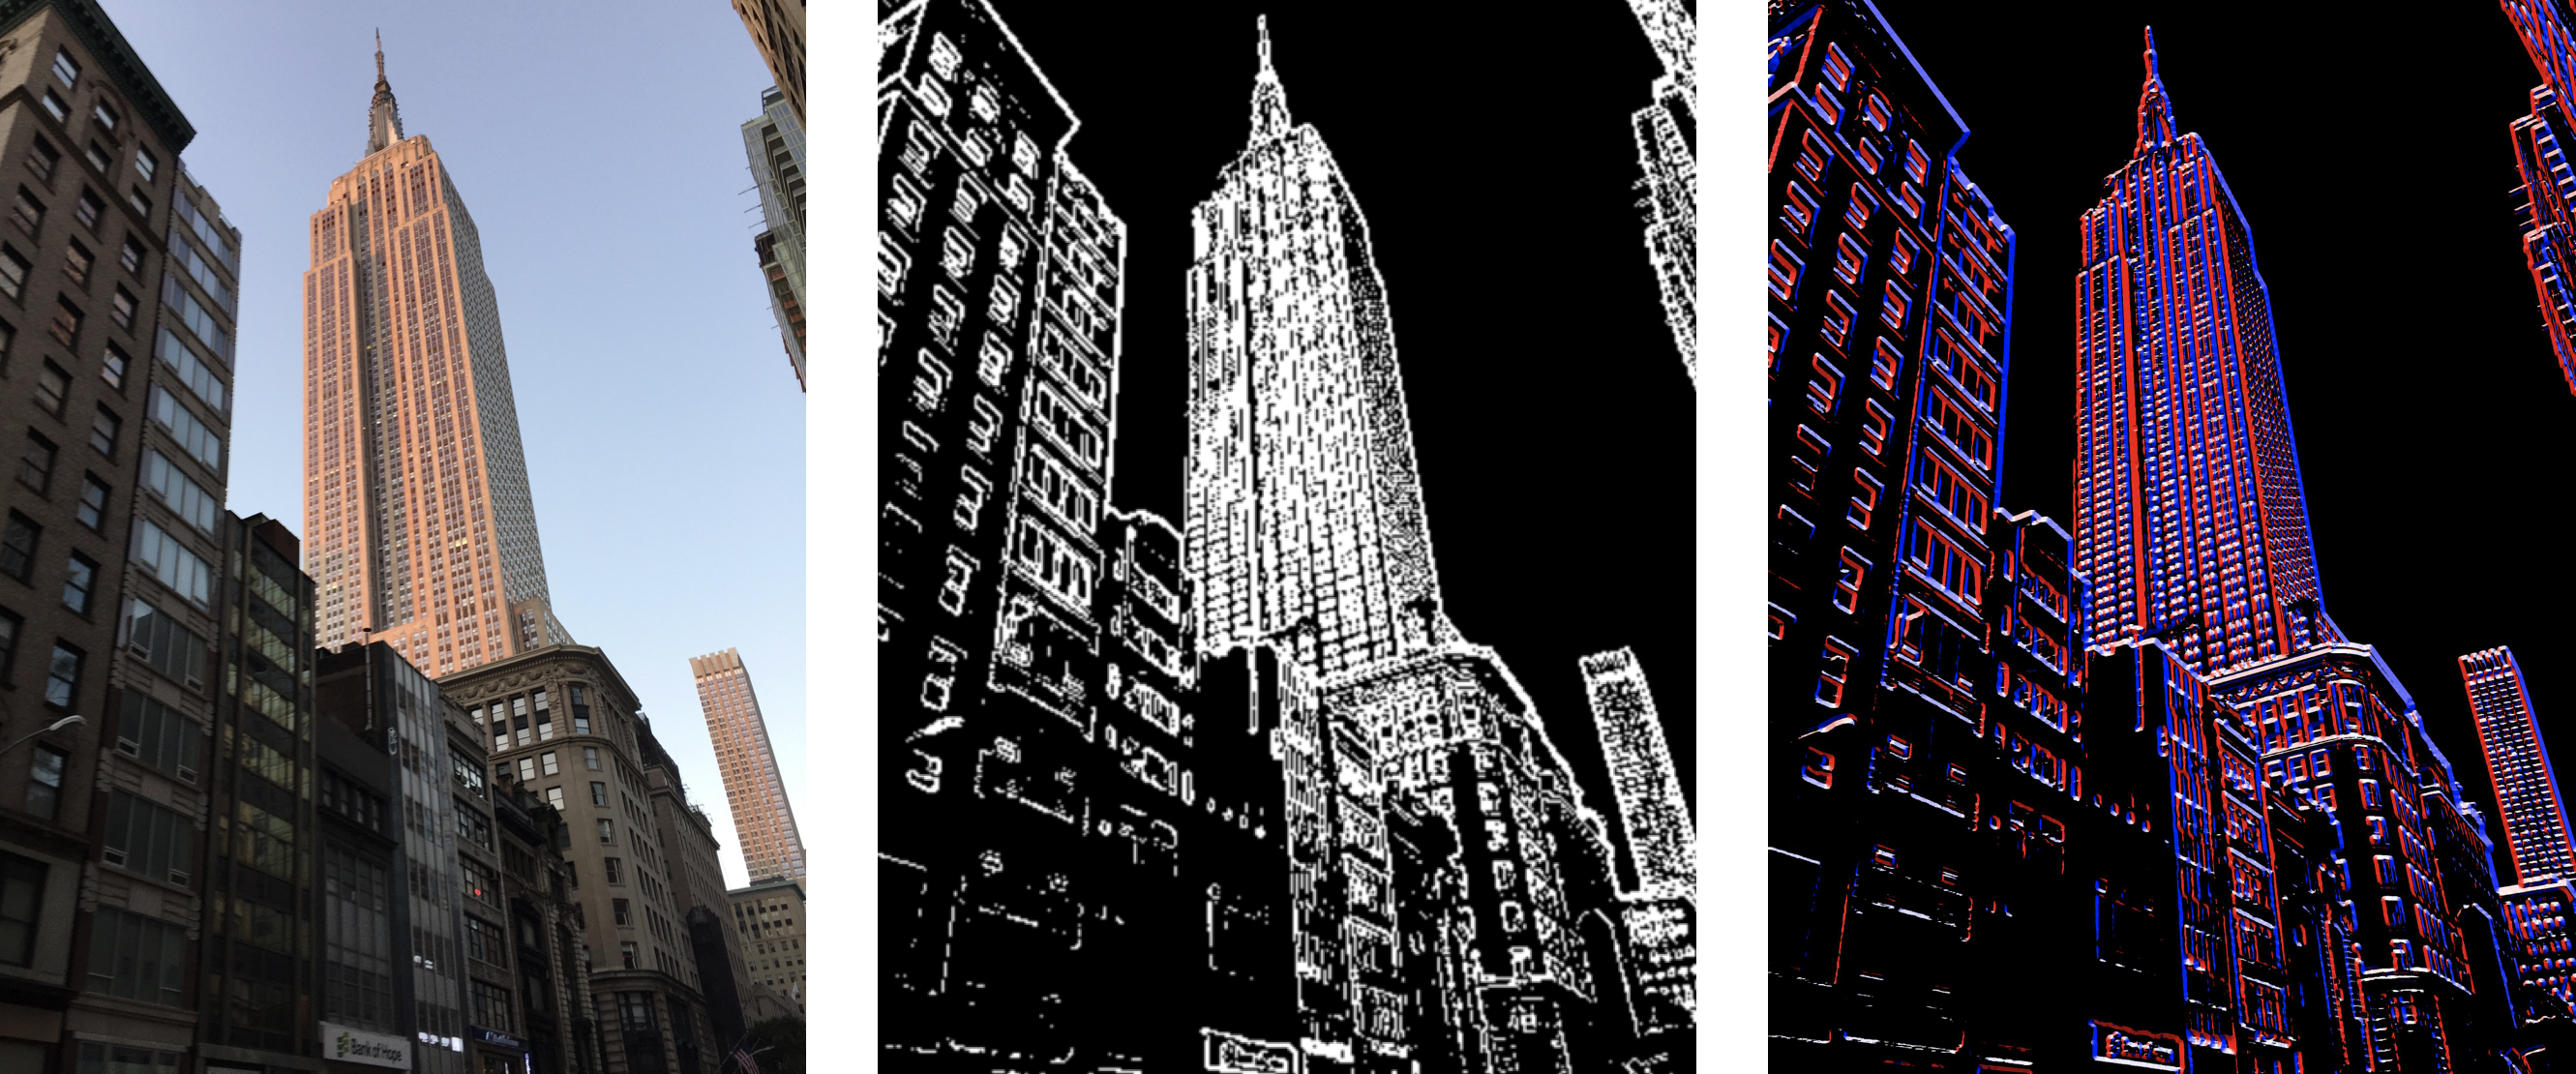
\includegraphics[height=5.8cm]{images/example_edge_coloring.png}
\caption{A demonstration of the approach. Left: the original image. Middle: the image gradient magnitude. Right: the image gradient magnitude pseudo-colored by the image gradient direction.}
\label{fig:example}
\end{figure}

\section{Conclusion}

We have presented an algorithm to color the edges of an image artistically. This approach leverages both the gradient image magnitude and direction to color image edges. By enhancing image gradients with color, we can better visualize edges and create new artistic renderings of images.

\subsubsection*{Acknowledgments}

I would like to thank my mentors at Carnegie Mellon University for their support on this project. Specifically, I am thankful for Dr. Ioannis Gkioulekas' insightful and passionate instruction in his Computer Vision class. I am also grateful to Dr. Eunsu Kang and Dr. Barnabas Poczos, whose Art and Machine Learning class provided a venue for arts-computing projects such as this one.

\bibliography{bib}

\section{Appendix}

\subsection{Examples of image edge coloring}

Here, we present a few examples of results from the edge coloring pipeline. The original images are shown on the left along with their colored image edges on the right.

\begin{figure}[h!]
\centering
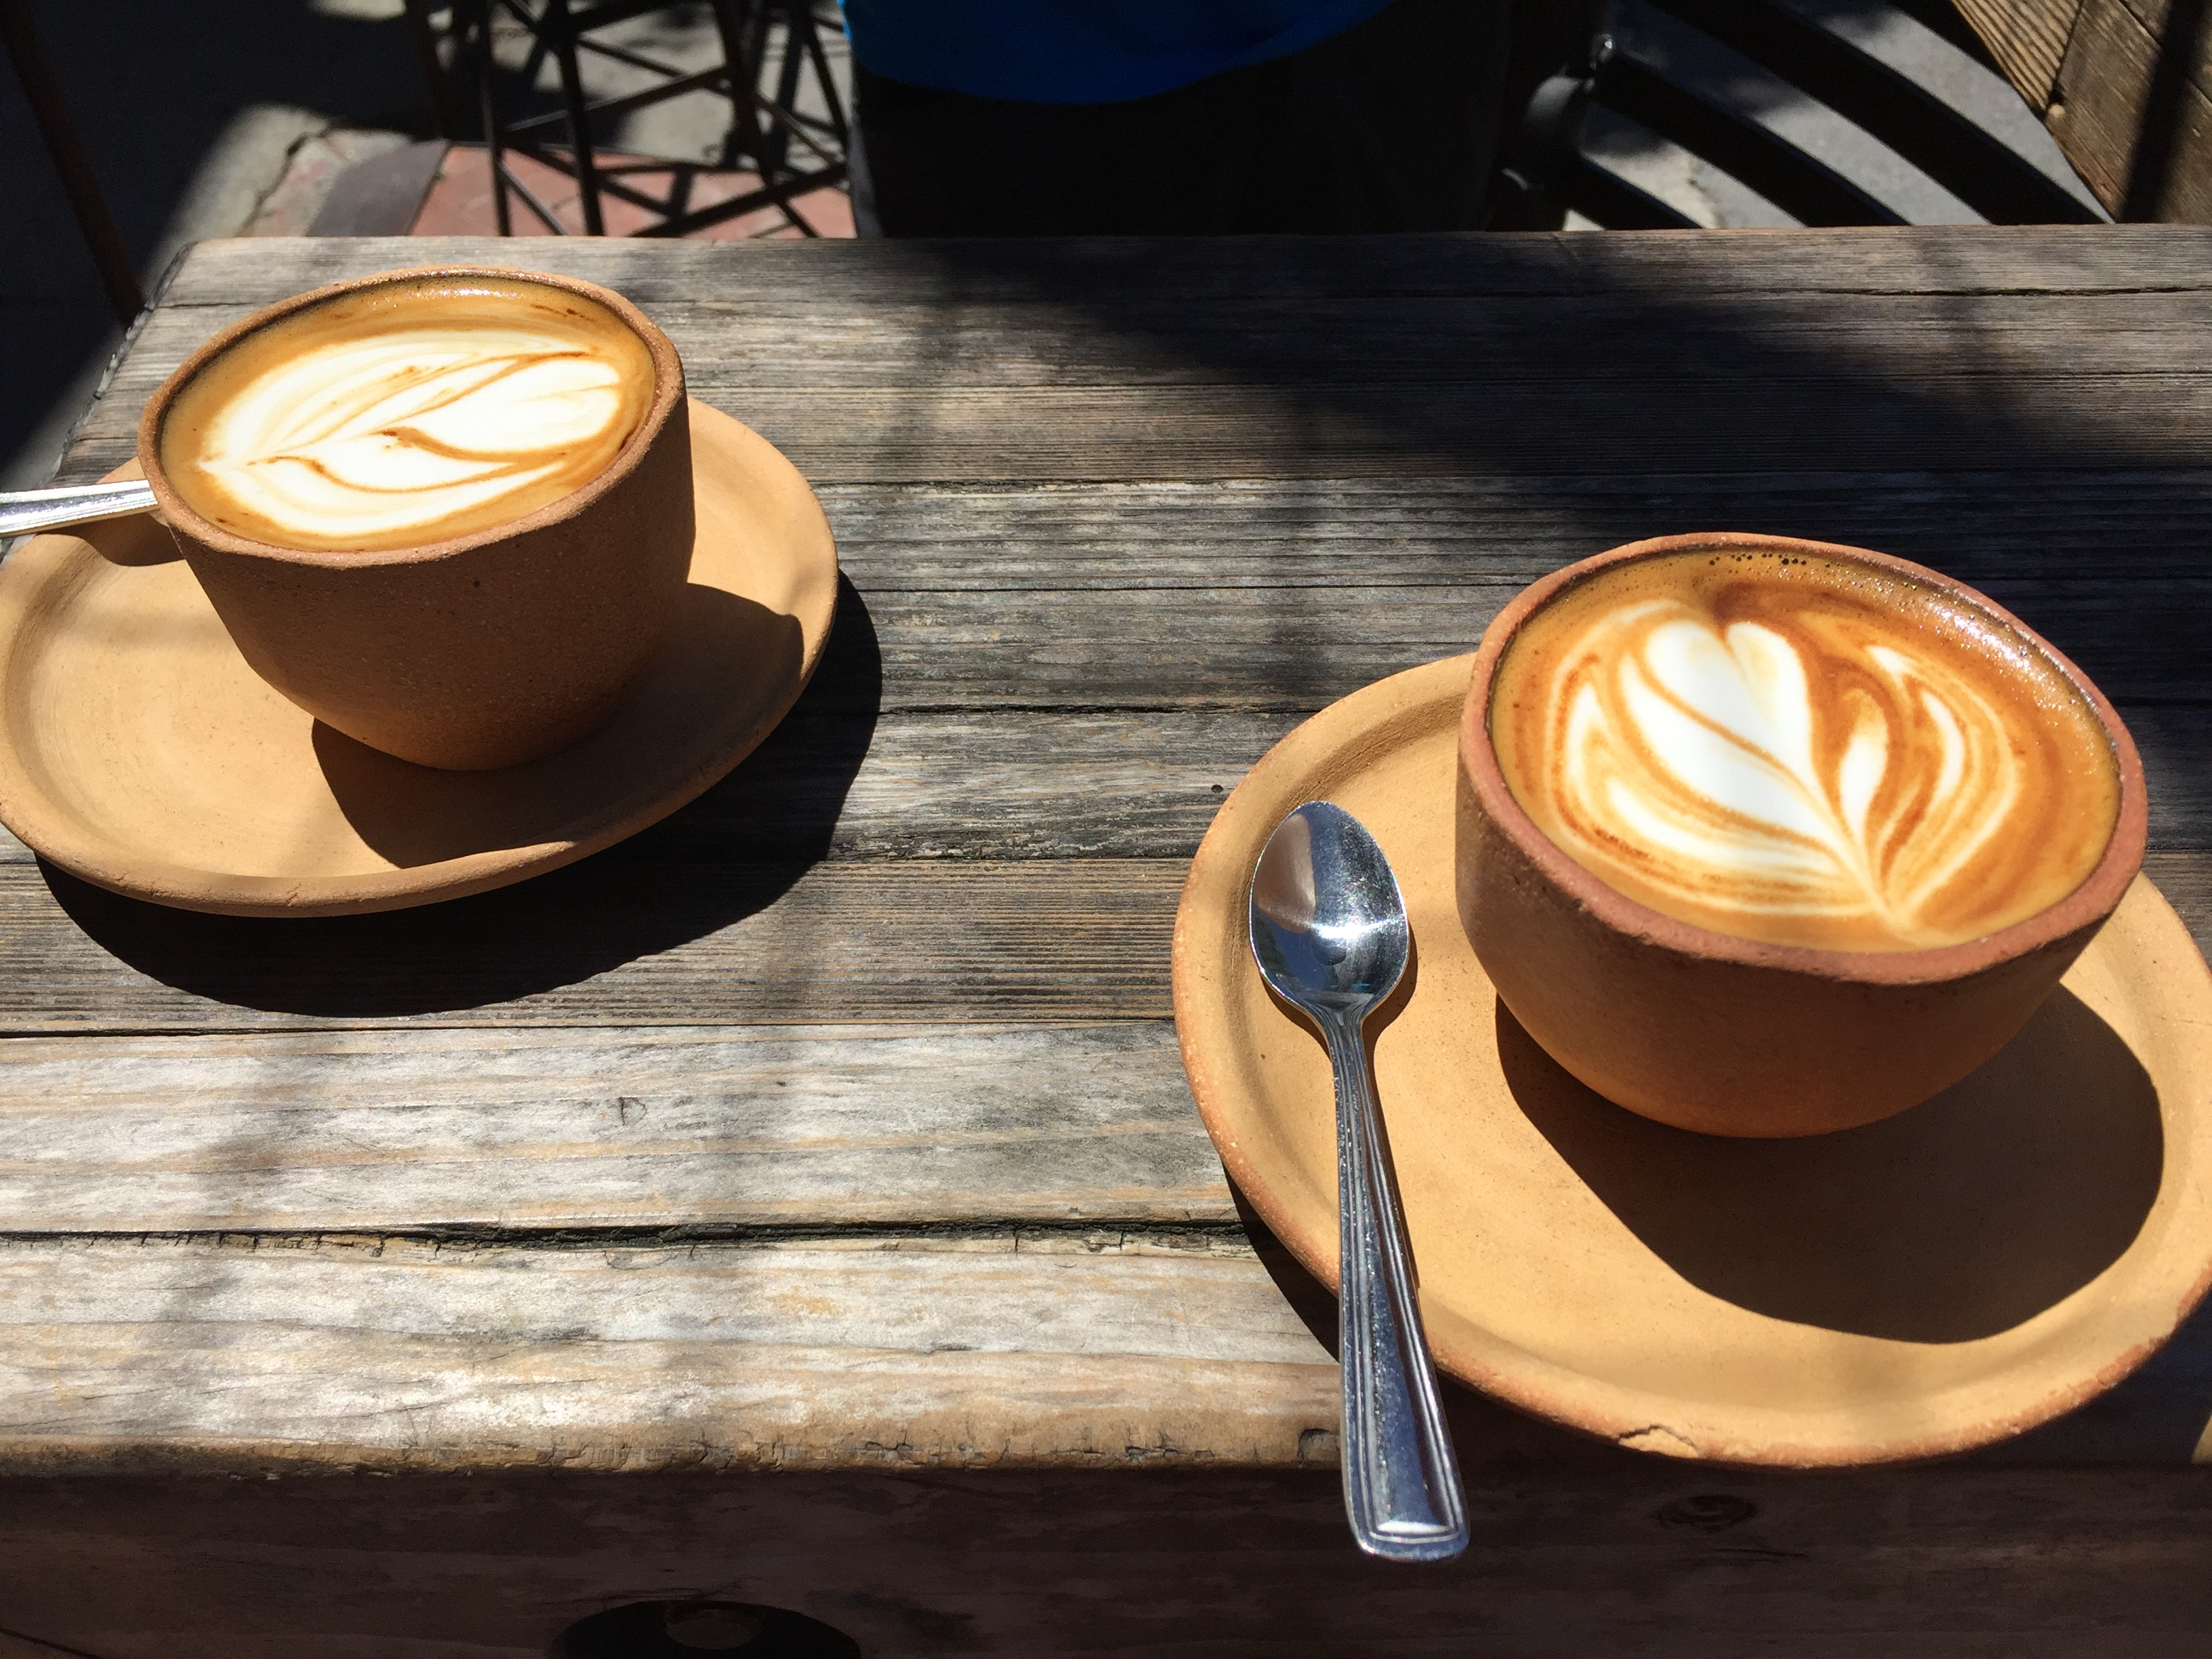
\includegraphics[height=5cm]{images/orig_1.jpg}
\hspace{0.4cm}
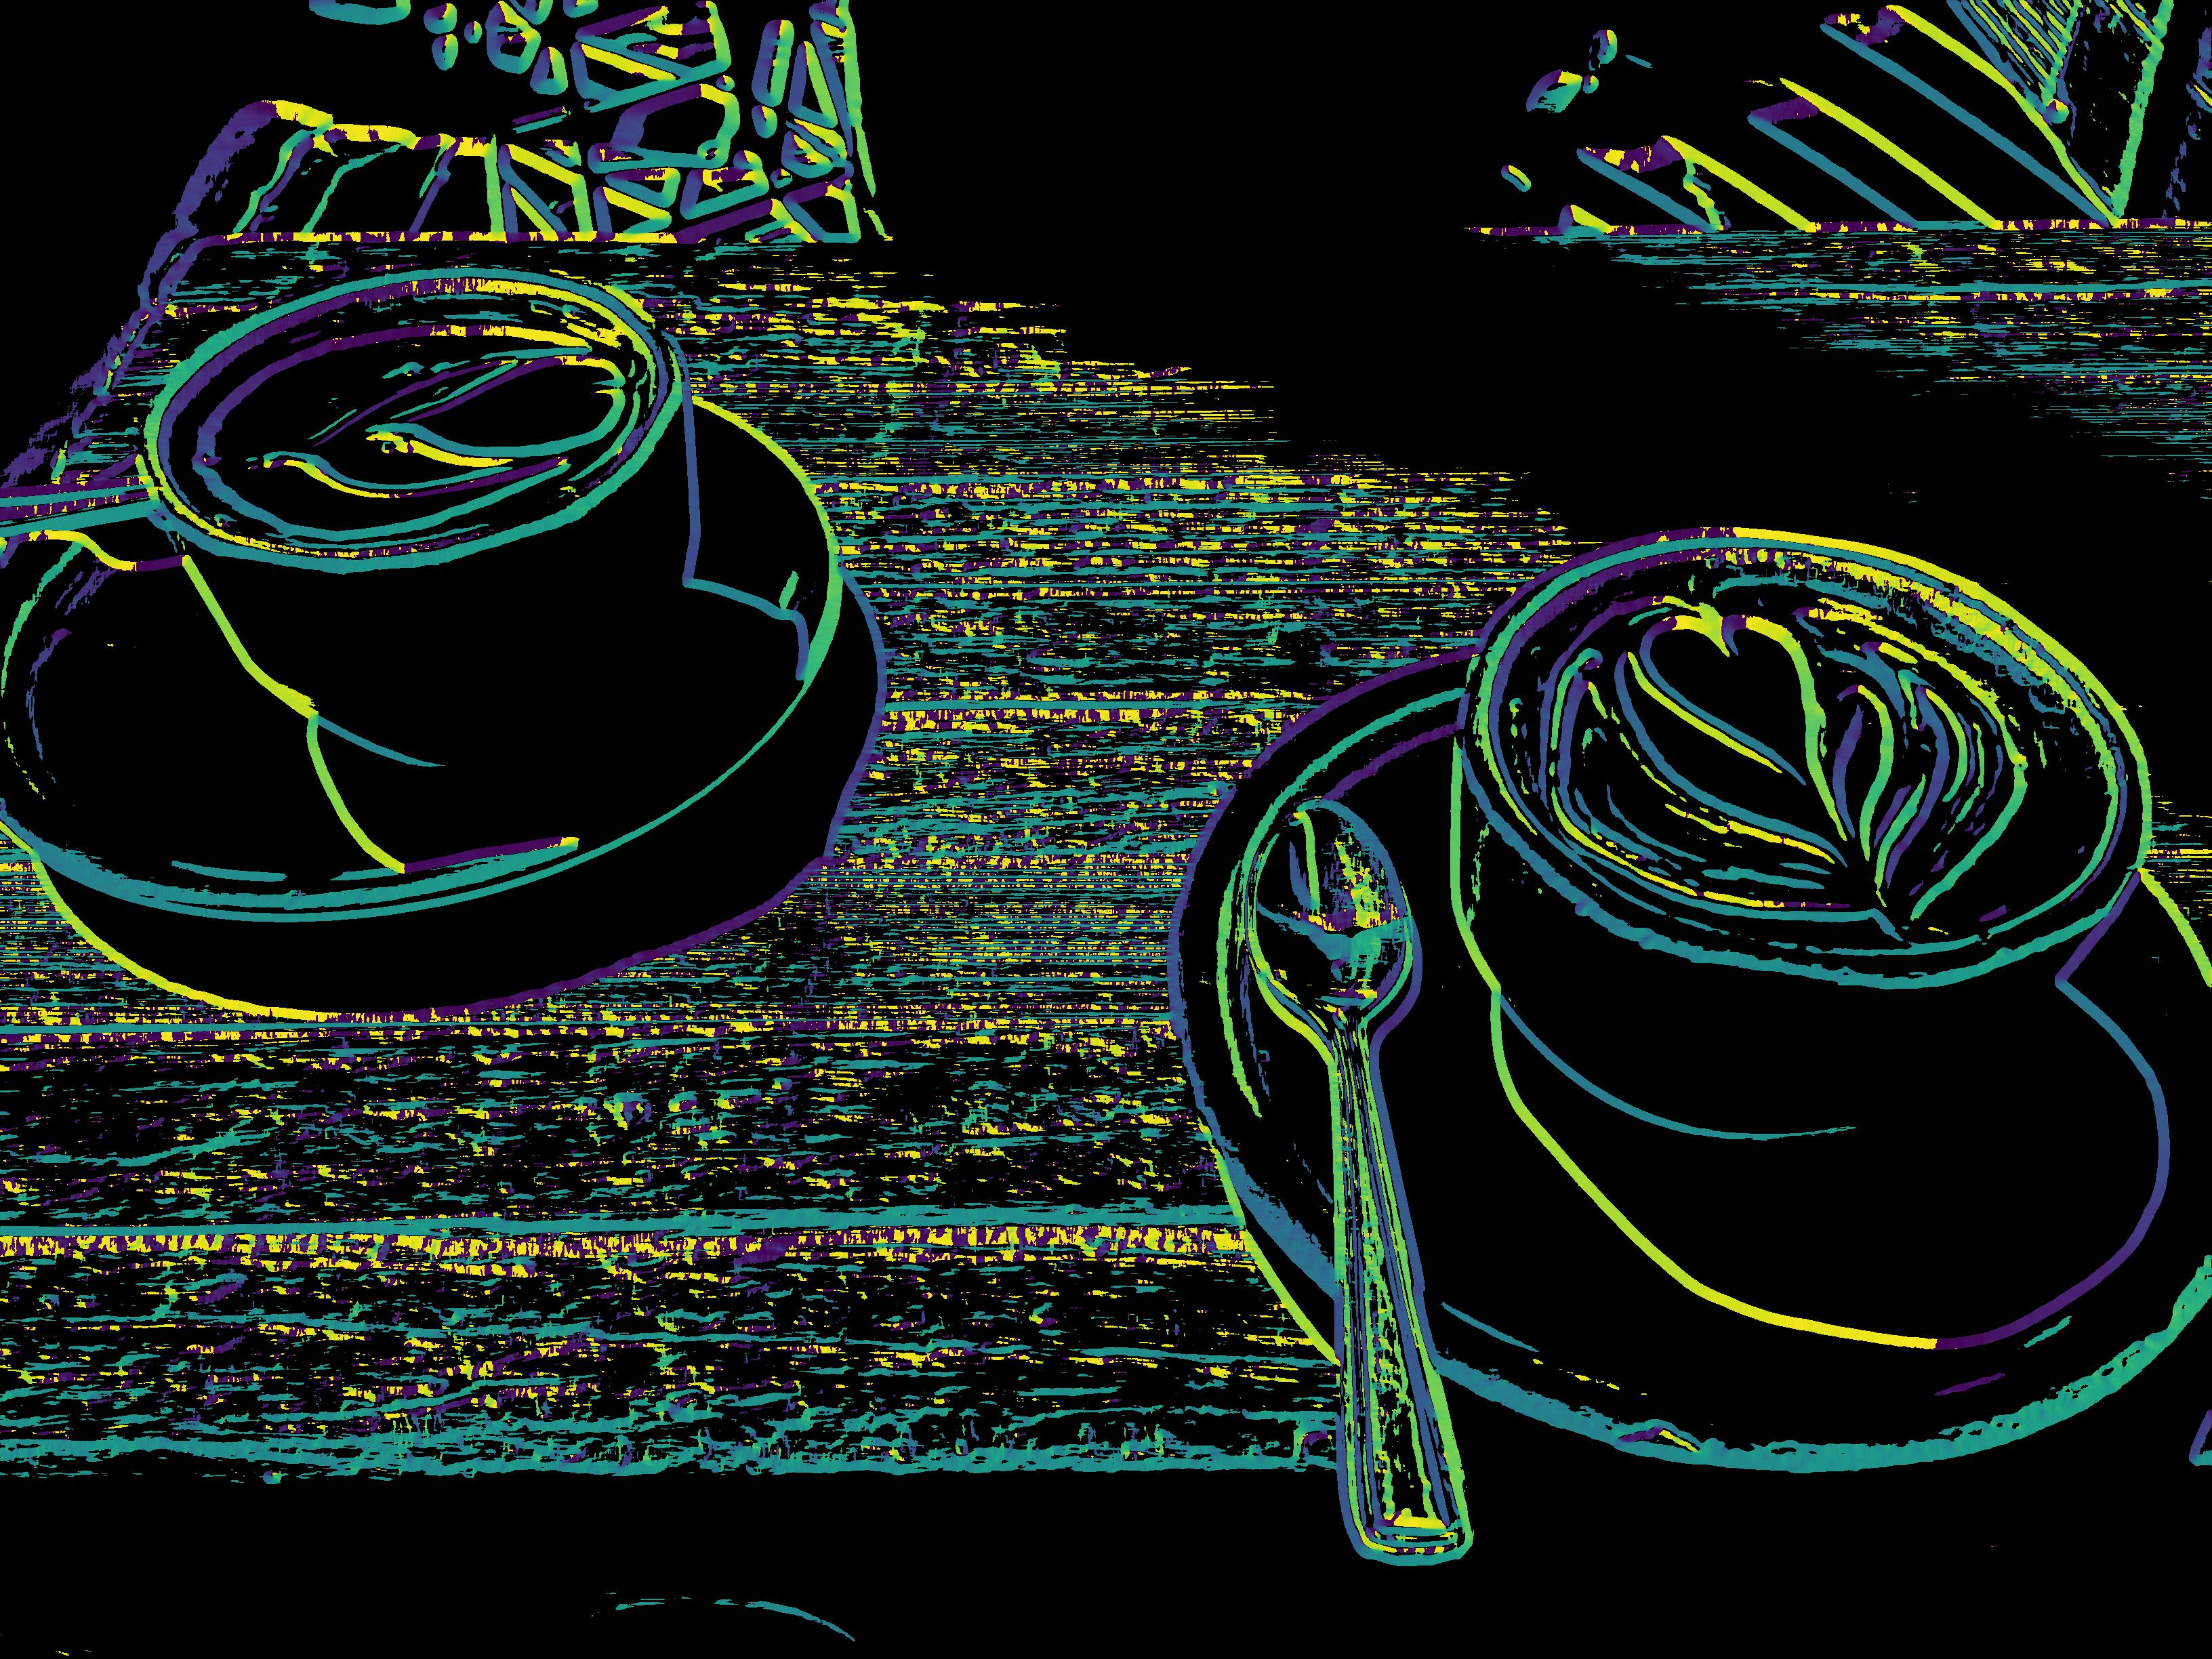
\includegraphics[height=5cm]{images/edge_color_1.jpg}
\end{figure}

\begin{figure}[h!]
\centering
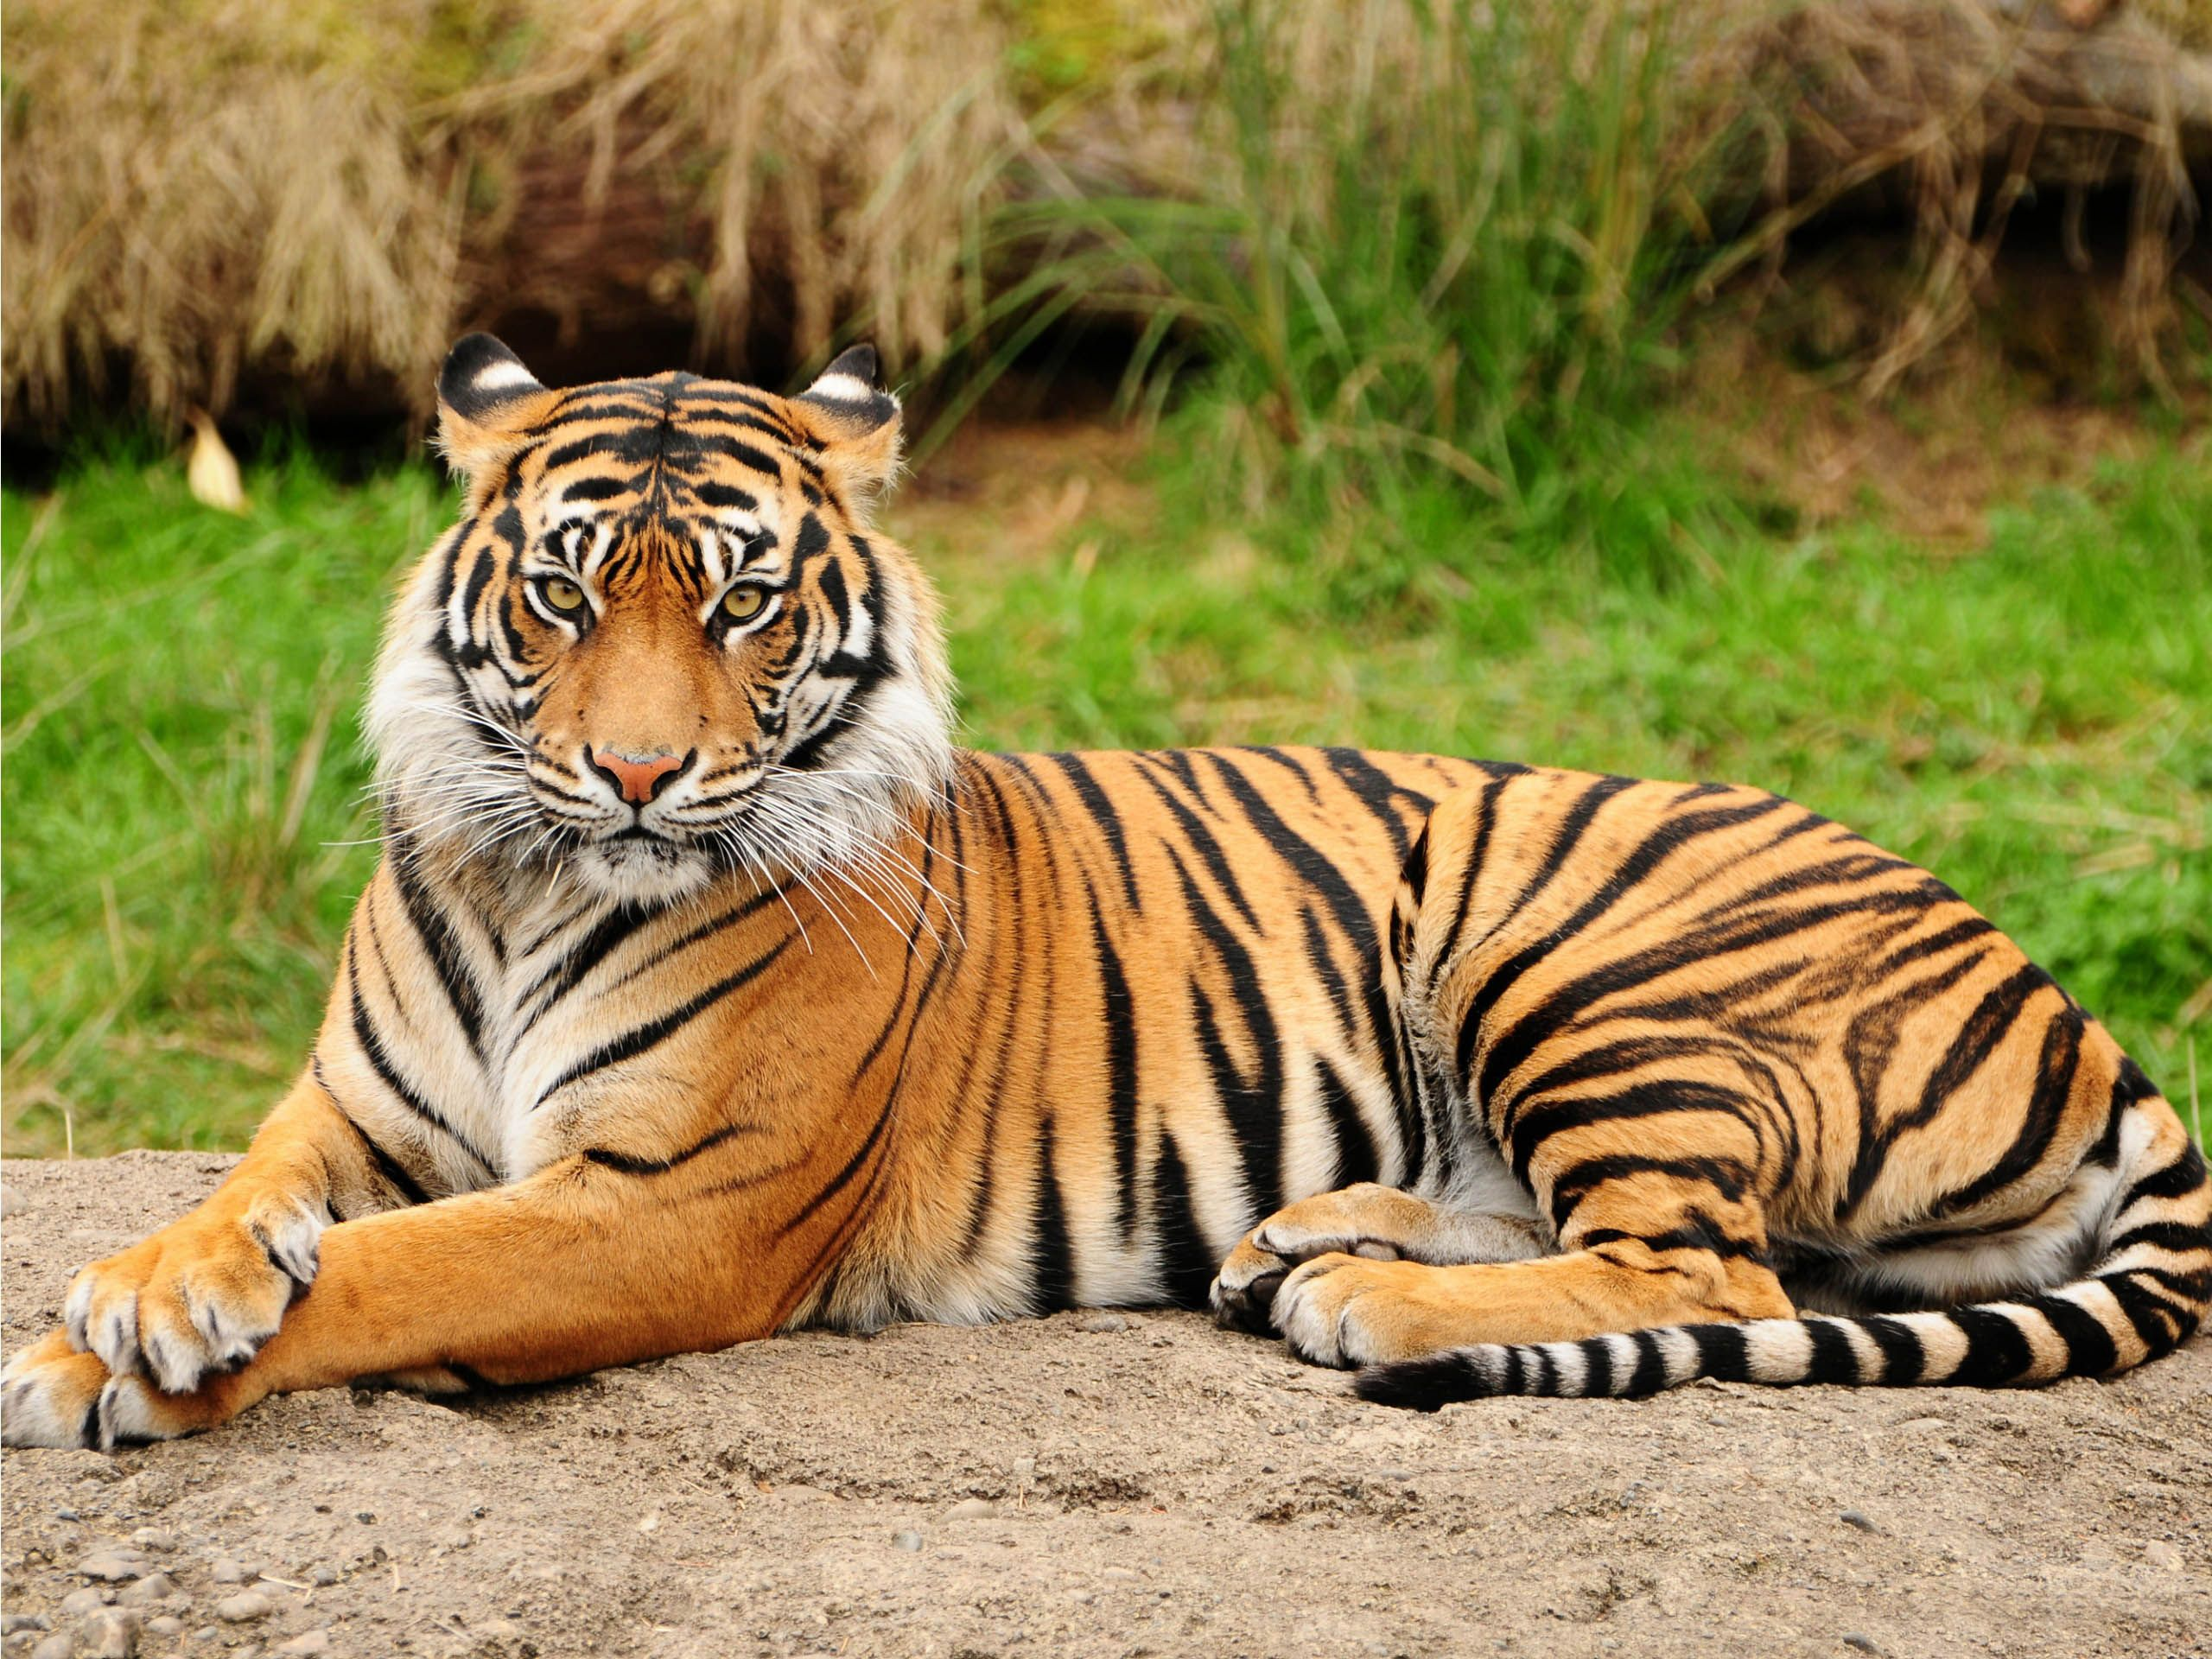
\includegraphics[height=5cm]{images/orig_2.jpg}
\hspace{0.4cm}
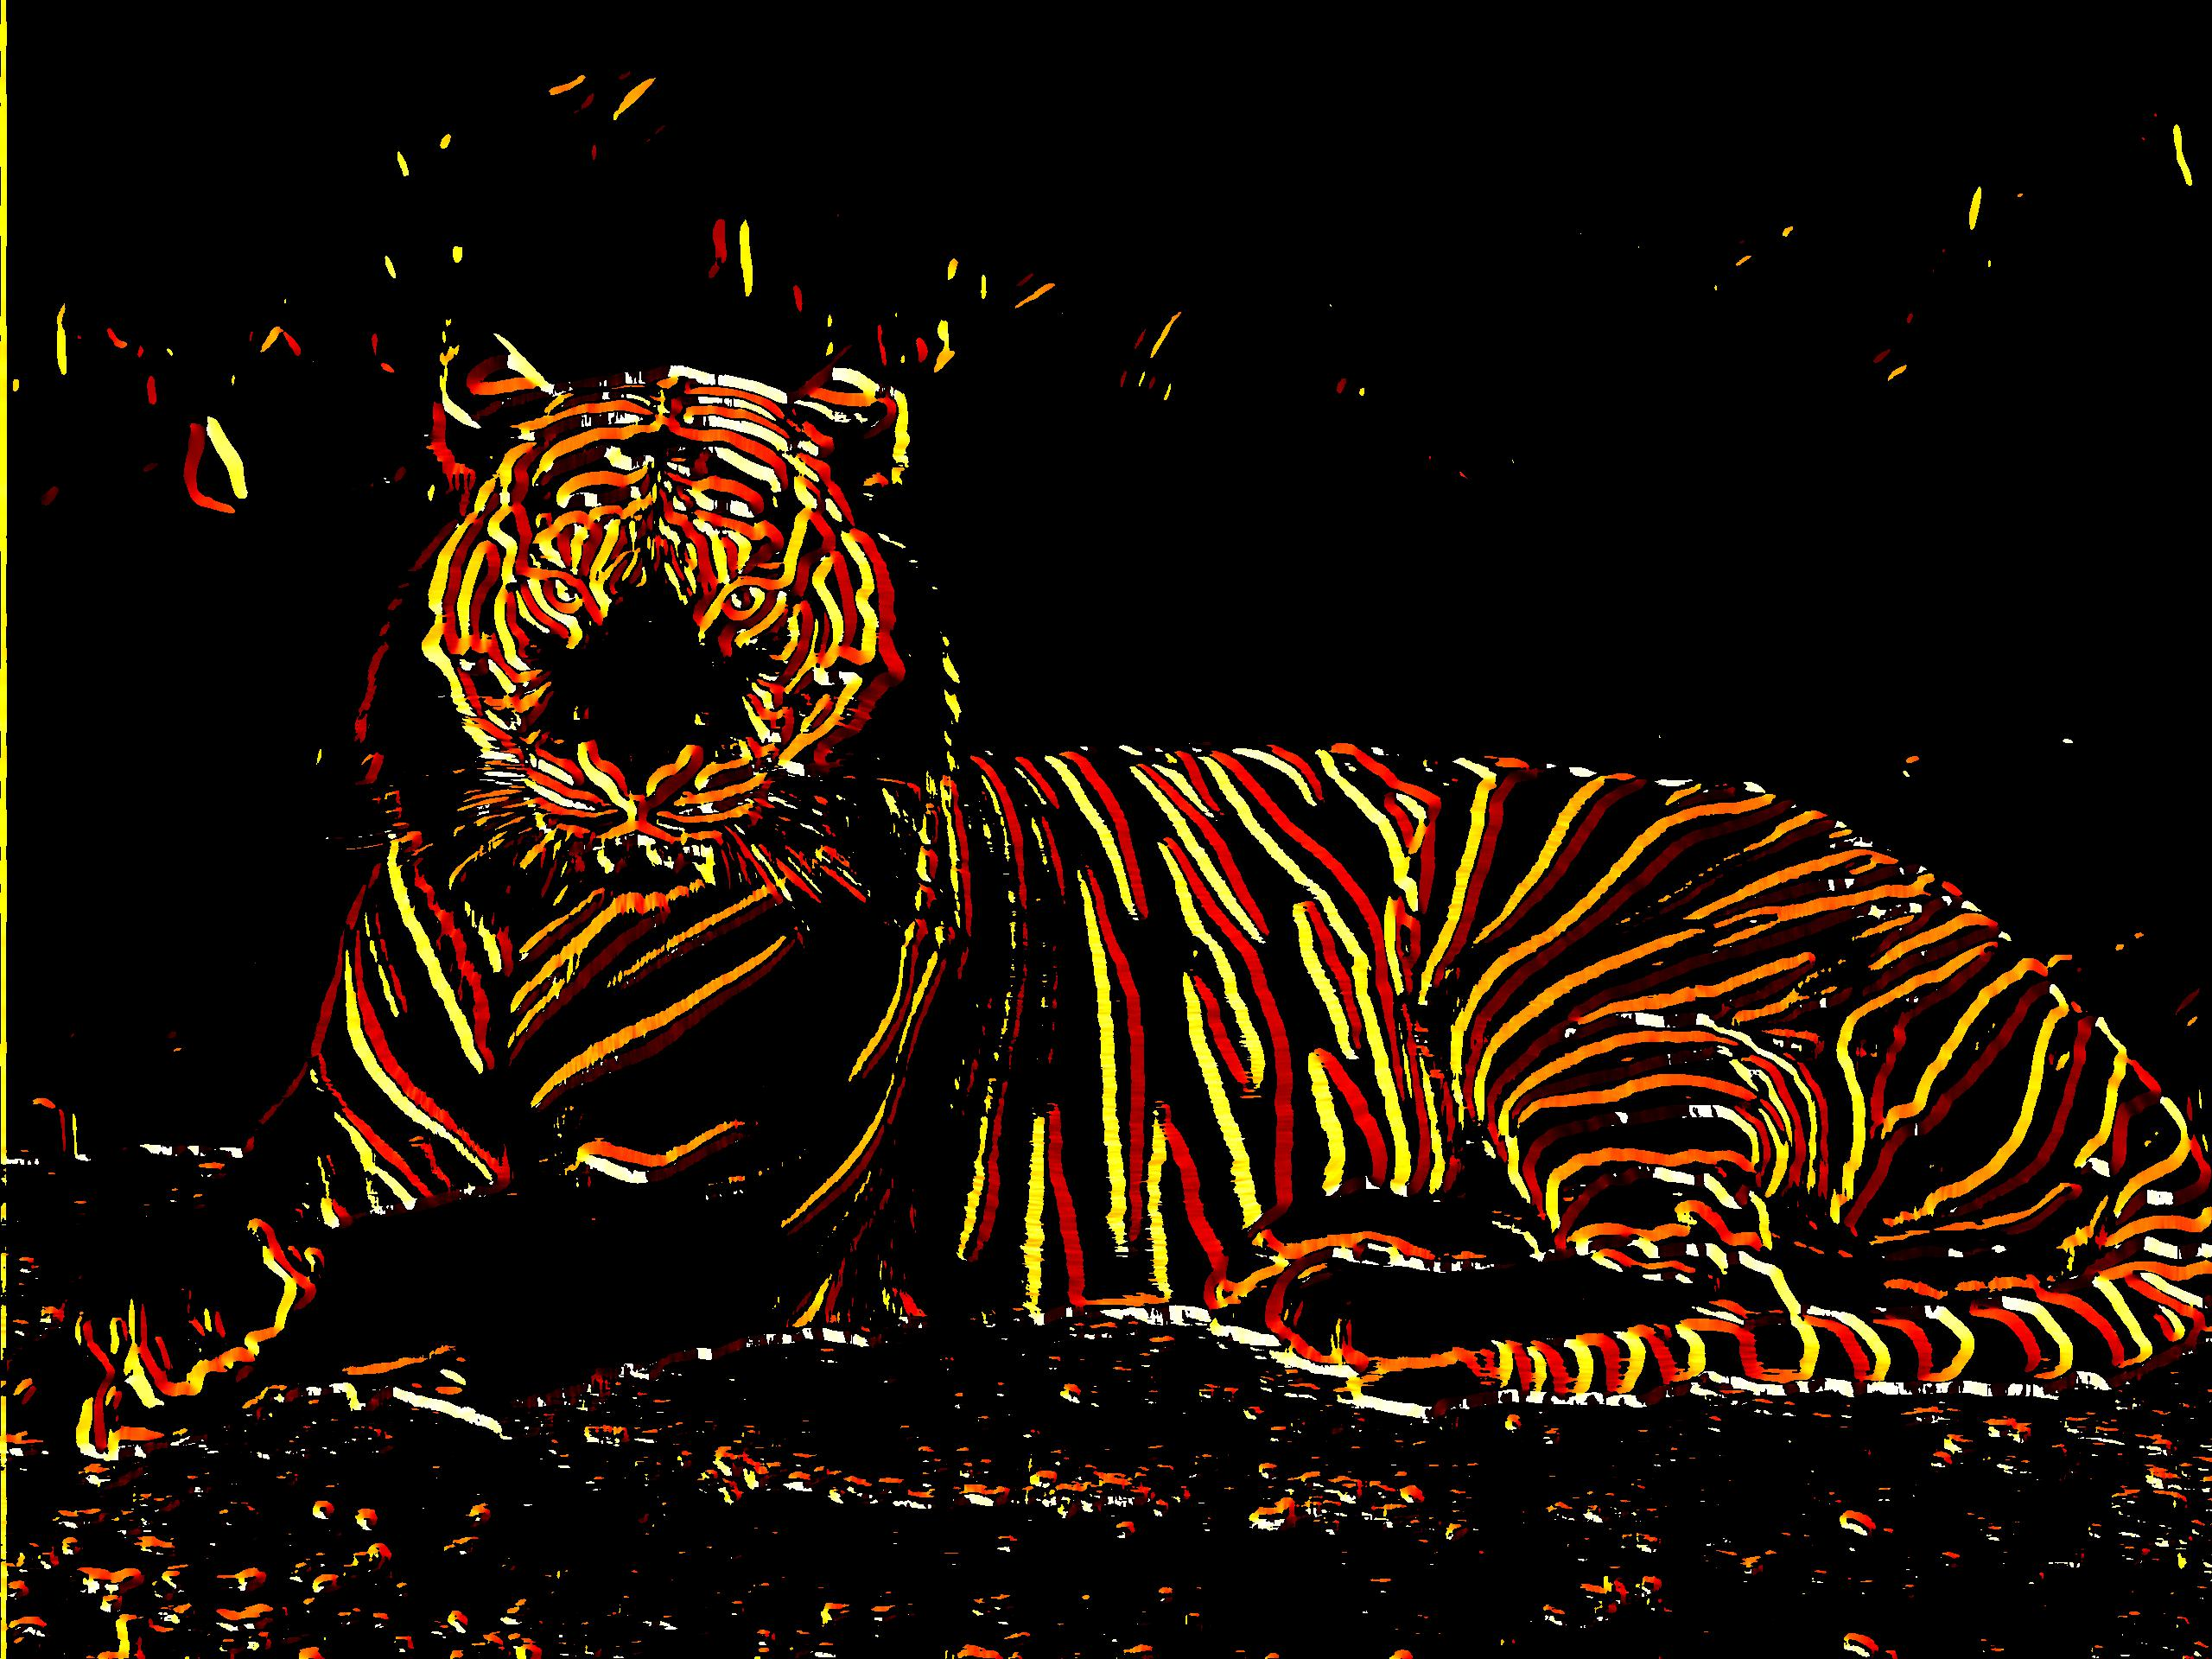
\includegraphics[height=5cm]{images/edge_color_2.jpg}
\end{figure}

\begin{figure}[h!]
\centering
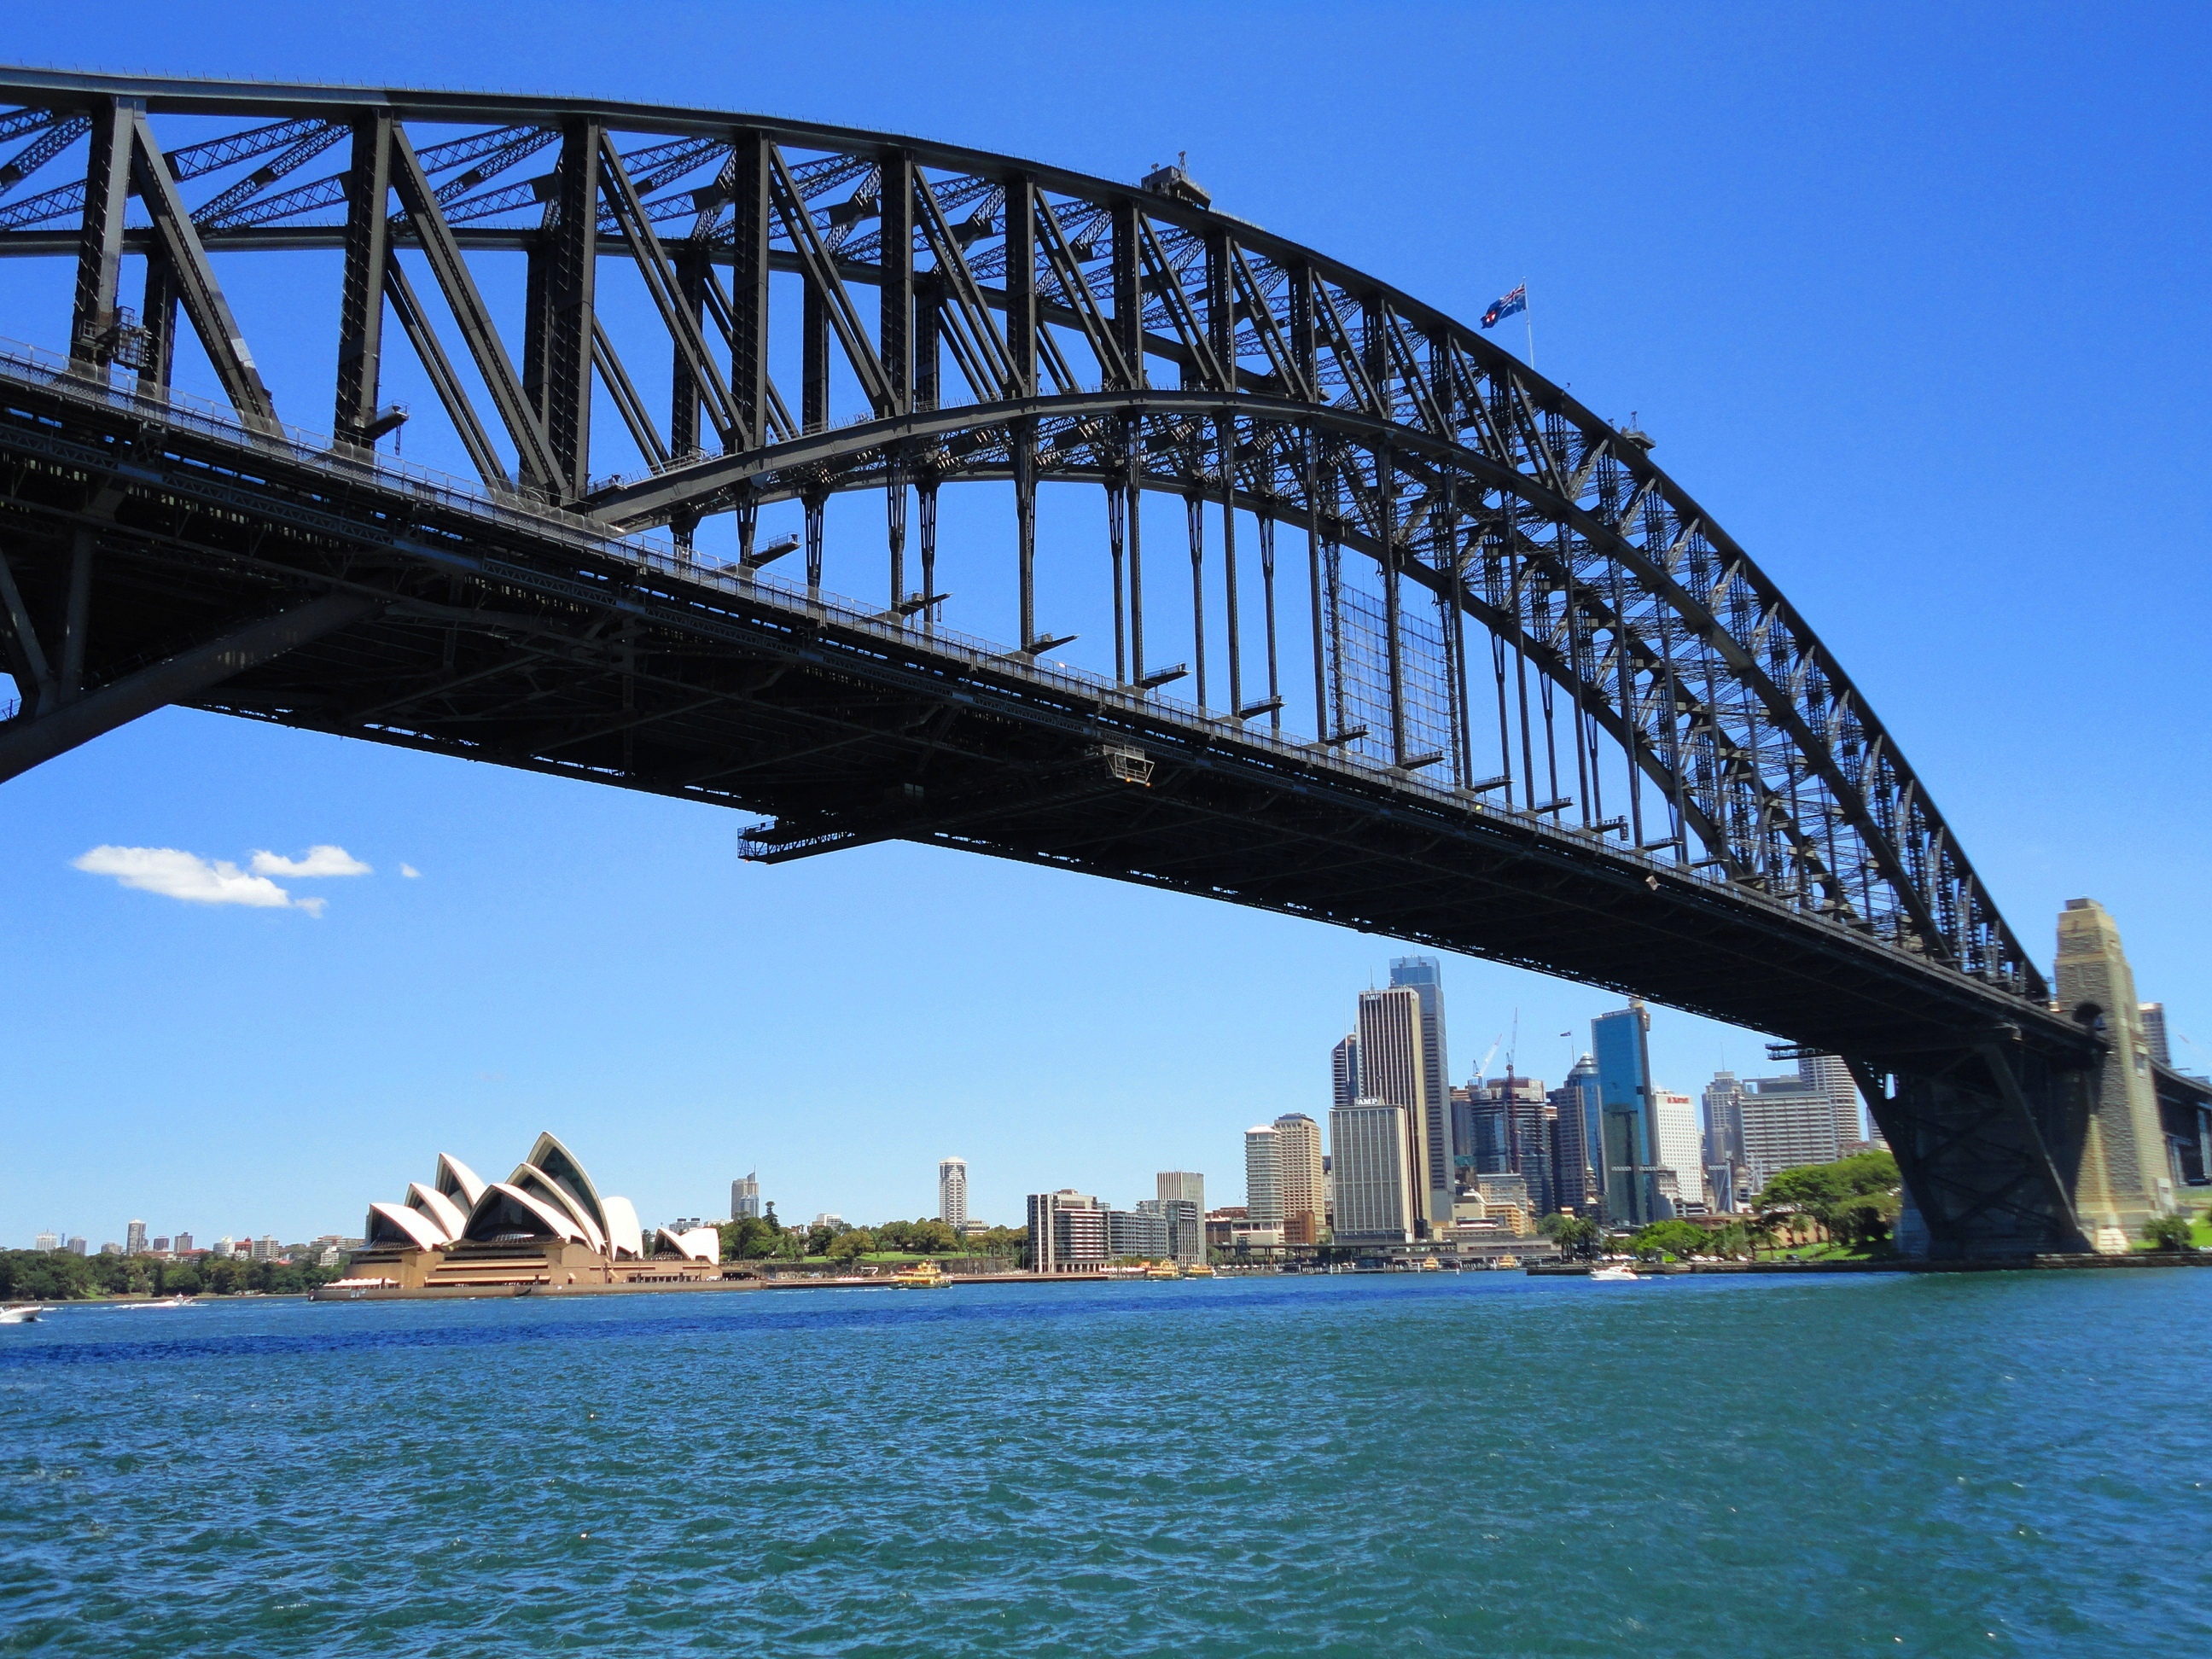
\includegraphics[height=5cm]{images/orig_3.jpg}
\hspace{0.4cm}
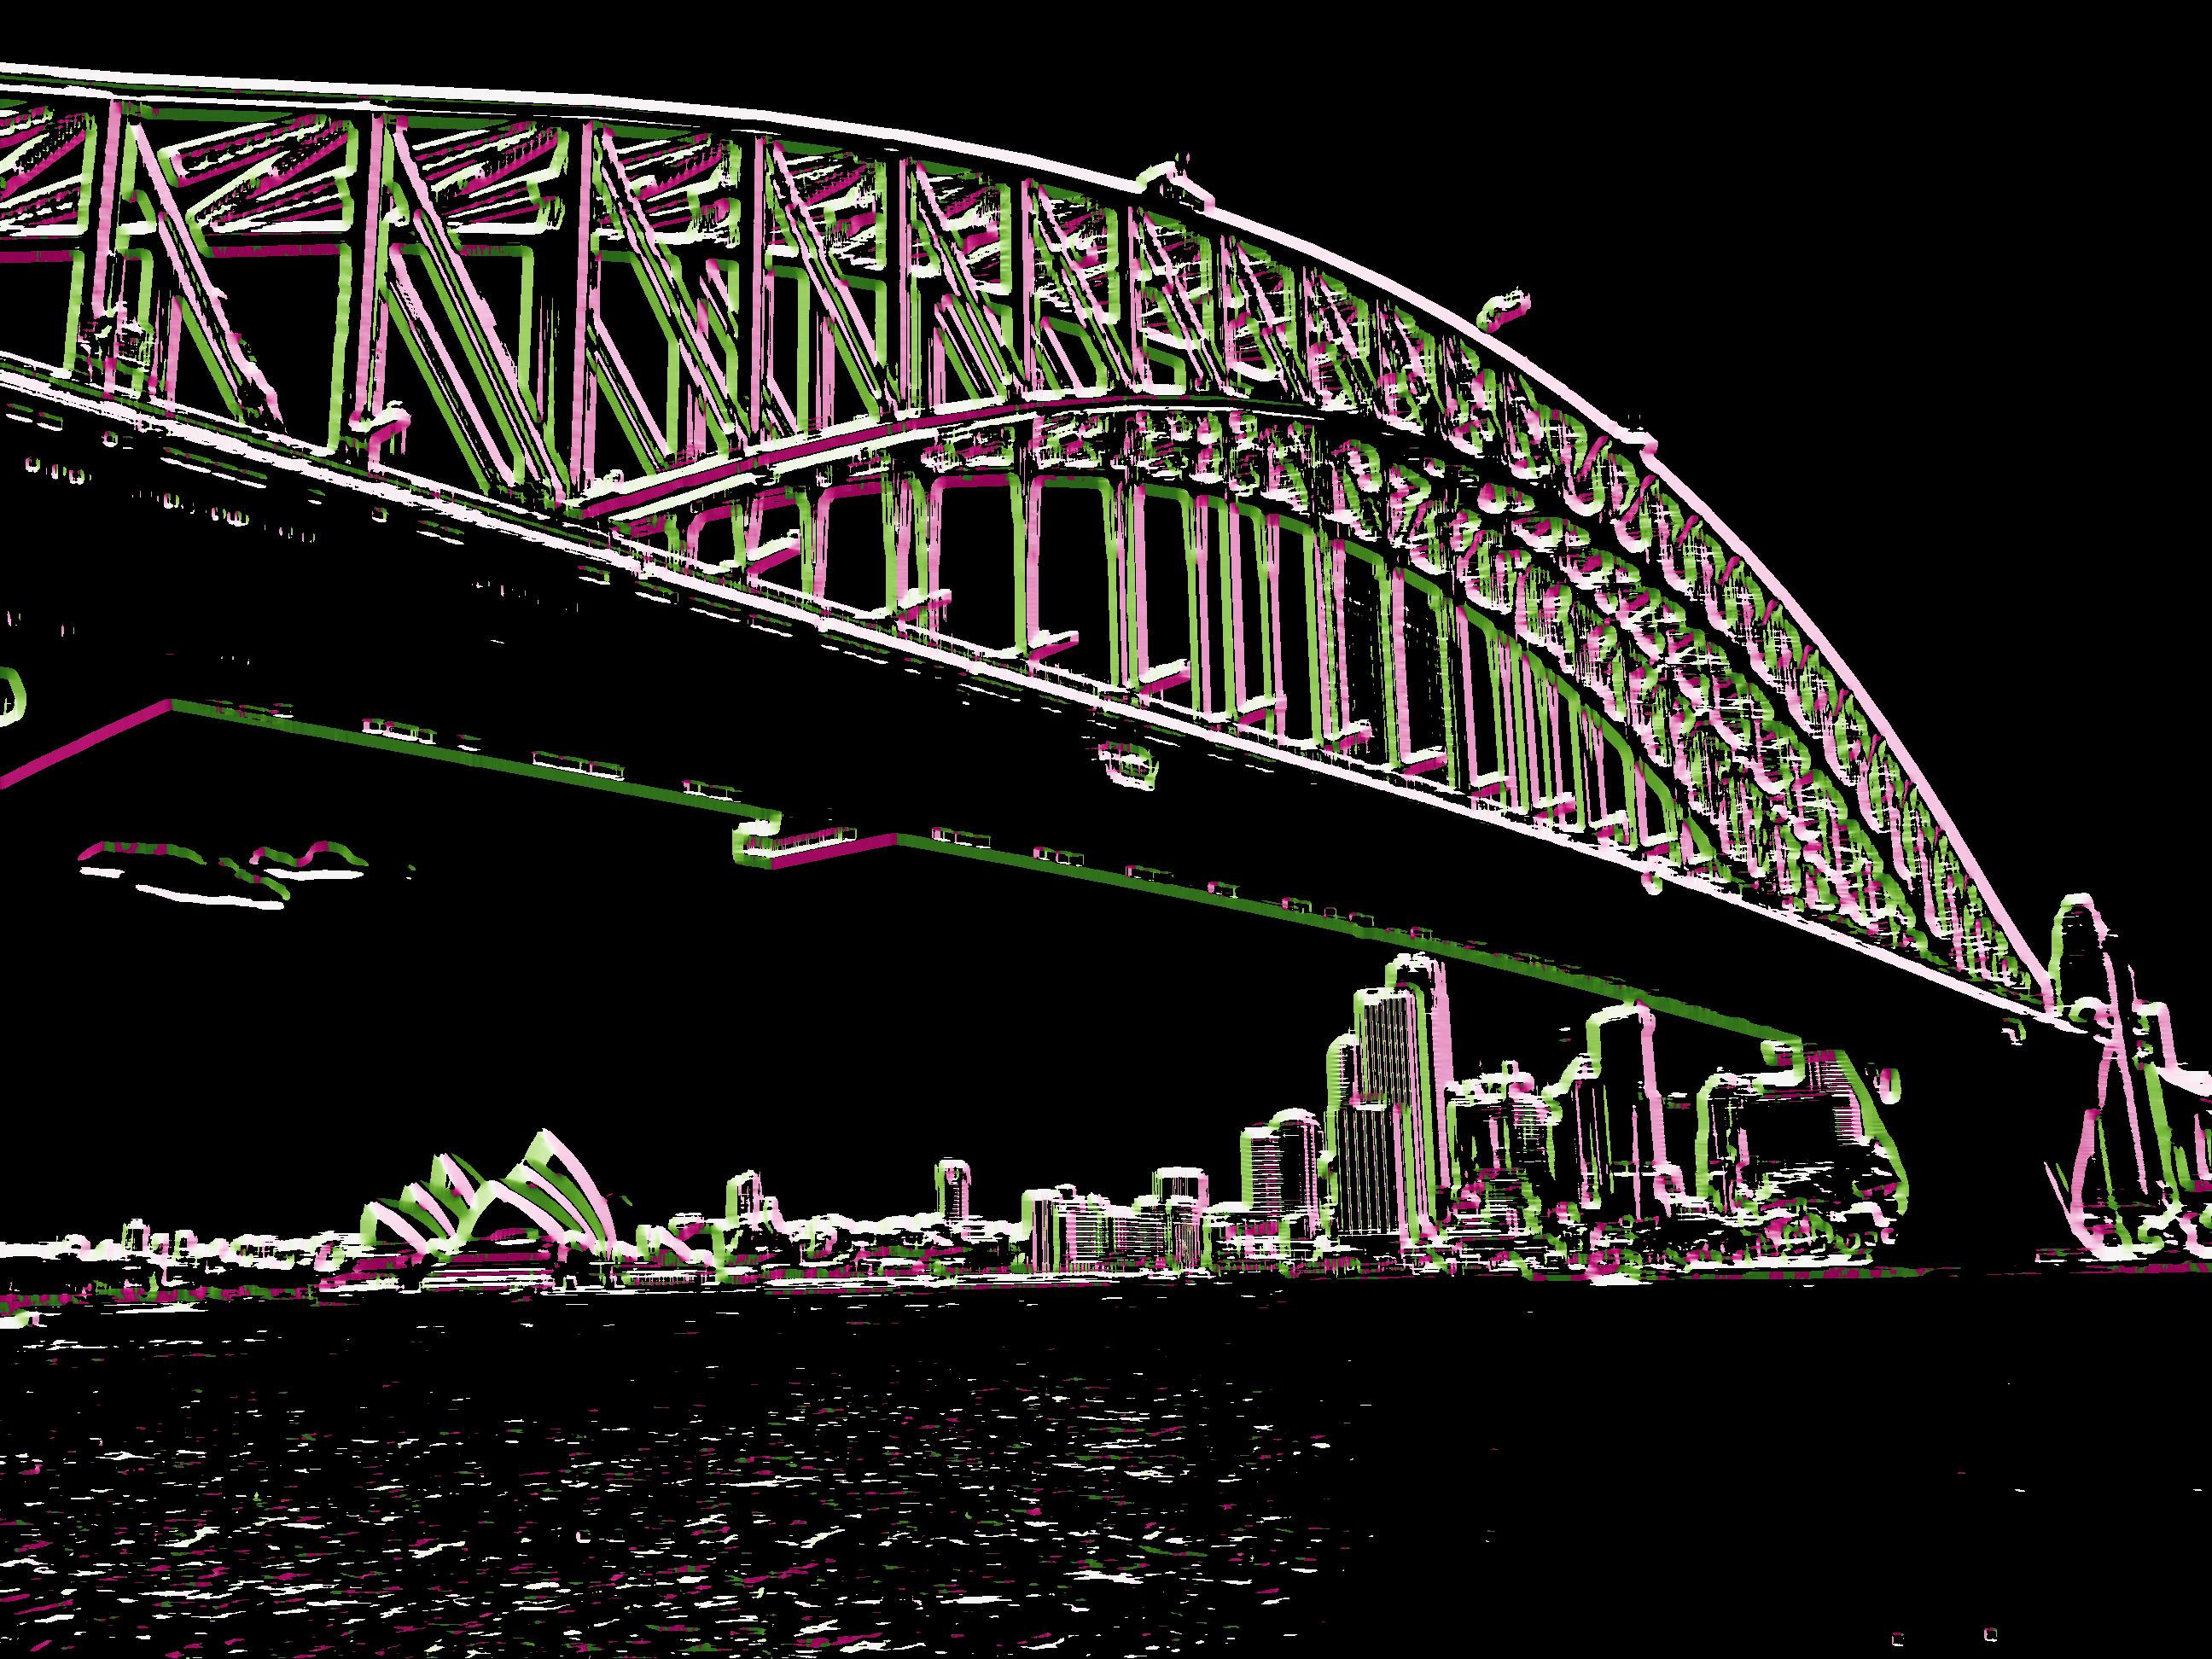
\includegraphics[height=5cm]{images/edge_color_3.jpg}
\end{figure}

\begin{figure}[h!]
\centering
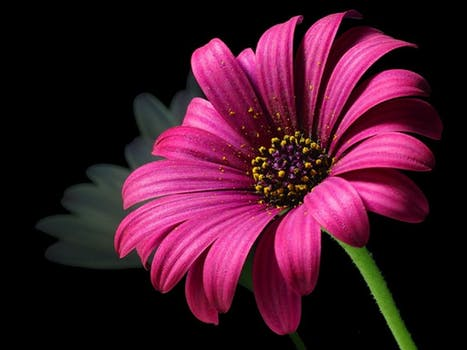
\includegraphics[height=5cm]{images/orig_4.jpg}
\hspace{0.4cm}
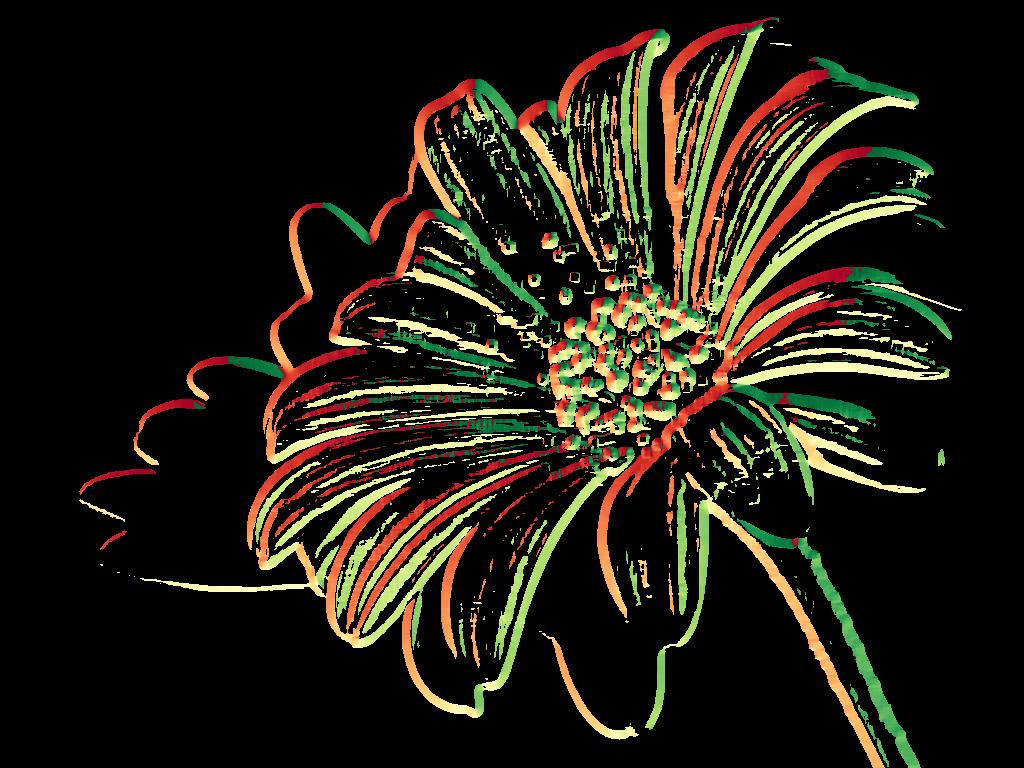
\includegraphics[height=5cm]{images/edge_color_4.jpg}
\end{figure}

\subsection{Edge detection}

The standard approach for edge detection is to convolve an image with a derivative filter like the Sobel filter to differentiate the intensity of the image pixels with respect to the horizontal and vertical directions of the image. However, since differentiation is very sensitive to noise, it is useful to blur the image first \cite{filtering_lecture}. This can be achieved by convolving the original image $f$ with a blur filter, such as the Gaussian filter, to produce a blurred image $f_b$. For the purposes of edge detection, we will first convert $f$ to a grayscale image. Figure 2 shows the blur transformation.

\begin{align}
f_b = f * \frac{1}{16} \begin{bmatrix} 
1 & \quad 2 & \quad 1 \\ 
2 & \quad 4 & \quad 2 \\ 
1 & \quad 2 & \quad 1  
\end{bmatrix}
\end{align}

\begin{figure}[h!]
\centering
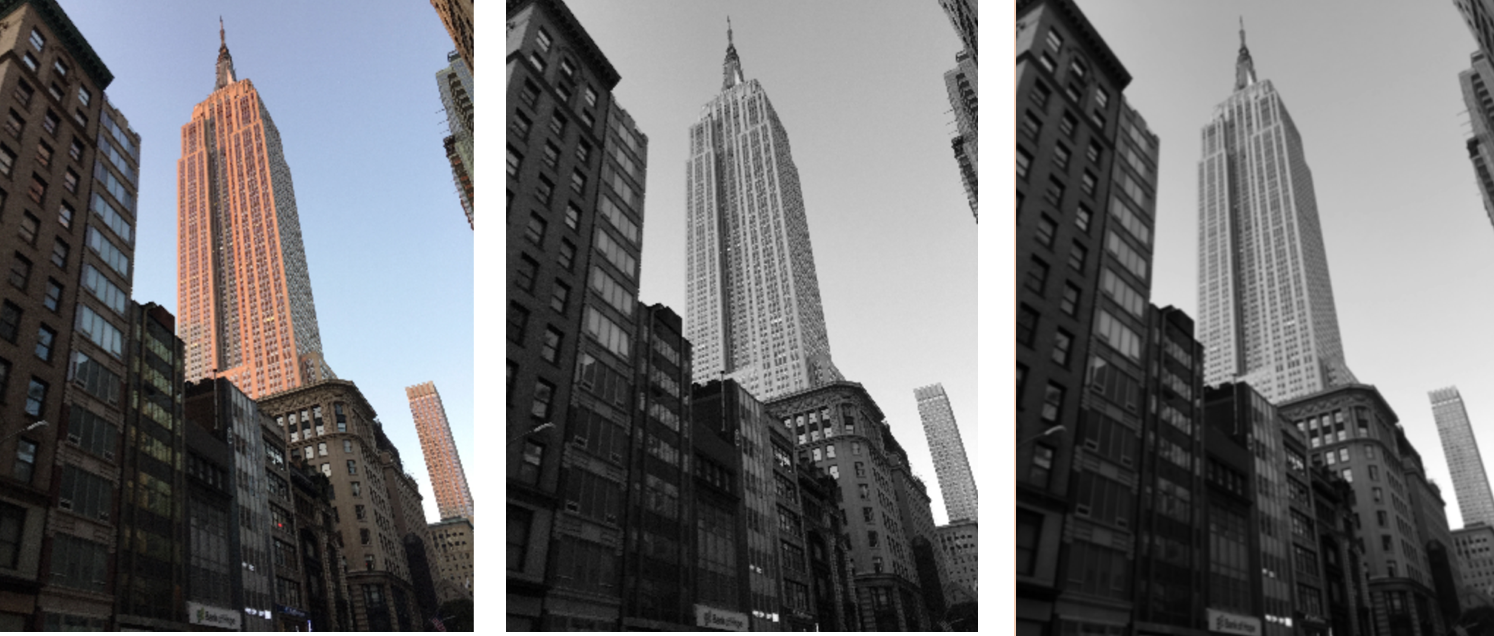
\includegraphics[height=5cm]{images/blur.png}
\caption{Blurring denoises the image and makes it easier to detect edges. The original image (left) is converted to grayscale (middle) and then blurred (right) using a blur filter.}
\label{fig:example}
\end{figure}

Once the image has been blurred, we can perform edge detection using Sobel filters \cite{sobel}. We convolve the blurred image $f_b$ with the horizontal and vertical Sobel filters, $S_x$ and $S_y$ respectively, to approximate the image derivatives in the horizontal and vertical directions, $\frac{\partial f_b}{\partial x}$ and $\frac{\partial f_b}{\partial y}$ respectively. $\frac{\partial f_b}{\partial x}$ has a strong response to vertical edges, and $\frac{\partial f_b}{\partial y}$ has a strong response to horizontal edges.

\begin{align}
S_x = \begin{bmatrix} 
1 & \quad 0 & \quad -1 \\ 
2 & \quad 0 & \quad -2 \\ 
1 & \quad 0 & \quad -1  
\end{bmatrix}
\quad S_y = \begin{bmatrix} 
1 & \quad 2 & \quad 1 \\ 
0 & \quad 0 & \quad 0 \\ 
-1 & \quad -2 & \quad -1  
\end{bmatrix}
\end{align}

\begin{align}
\frac{\partial f_b}{\partial x} &= f_b * S_x \\
\frac{\partial f_b}{\partial y} &= f_b * S_y
\end{align}

$\frac{\partial f_b}{\partial x}$ and $\frac{\partial f_b}{\partial y}$ can be combined to form the image gradient $\nabla f_b$. The following equations show how to compute the magnitude $G$ and direction $\theta$ of the image gradient. The resulting gradient magnitude represents the intensity of edges in the image and is displayed in Figure 3. 

\begin{align}
\nabla f_b &= \begin{bmatrix} \frac{\partial f_b}{\partial x}, \frac{\partial f_b}{\partial y} \end{bmatrix} \\
G &= \vert \vert \nabla f_b \vert \vert = \sqrt{\Big( \frac{\partial f_b}{\partial x} \Big)^2 + \Big( \frac{\partial f_b}{\partial y} \Big)^2} \\
\theta &= tan^{-1} \Big(\frac{\partial f_b}{\partial x} / \frac{\partial f_b}{\partial y}\Big)
\end{align}

\begin{figure}[h!]
\centering
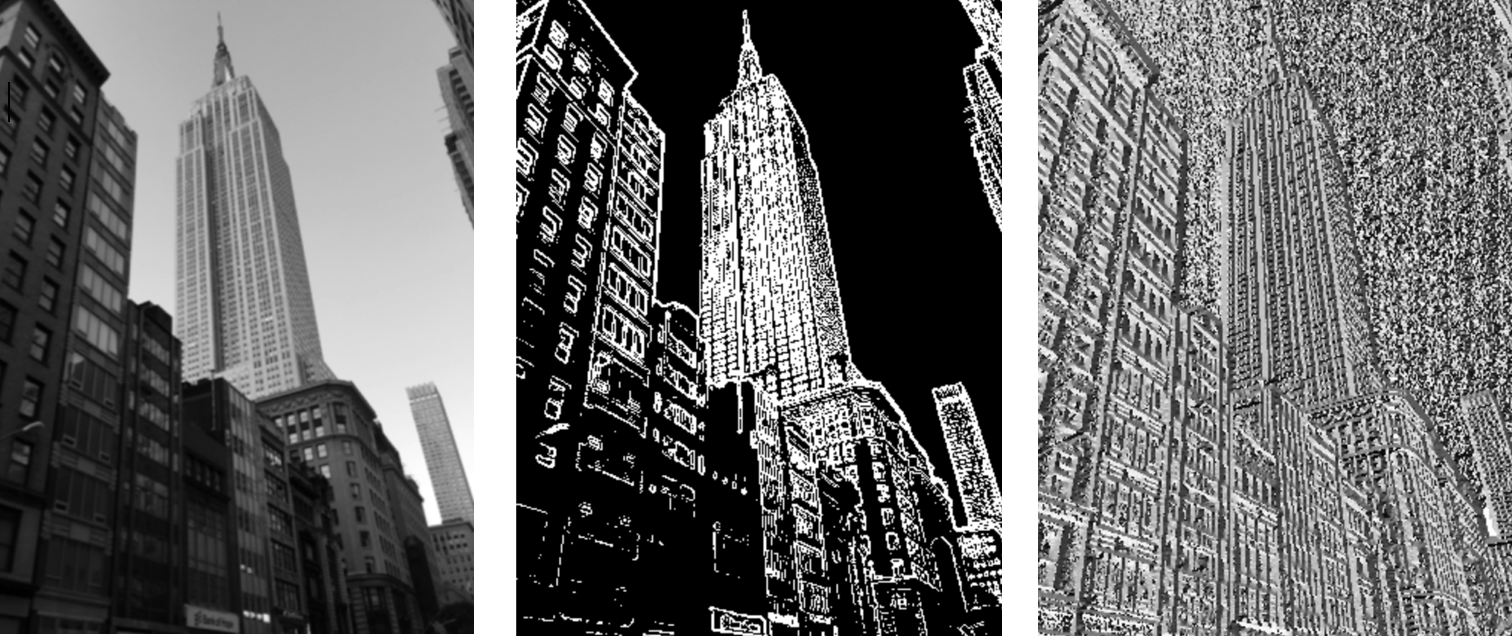
\includegraphics[height=5.5cm]{images/edge.png}
\caption{Edge detection using Sobel filters. We convolve the blurred image (left) with the Sobel filters and compute the magnitude (middle) and direction (right) of the image gradient.}
\label{fig:example}
\end{figure}

\subsection{Code}

The code to reproduce these experiments is available in the following Jupyter Notebook: \url{https://github.com/shouvikmani/edge-colorizer/blob/master/edge_colorizer.ipynb}.

\end{document}